\chapter{Конструкторская часть}

В данном разделе будут приведены схемы алгоритма полного перебора и муравьиного алгоритма для решения задачи коммивояжера.

\section{Схема алгоритма полного перебора}

На рисунке \ref{fig:next_set} приведена cхема вспомогательной функции next\_set, которая позволяет сгенерировать все возможные перестановки первых n неотрицательных чисел.

\clearpage
\begin{figure}[h!]
	
	\centering{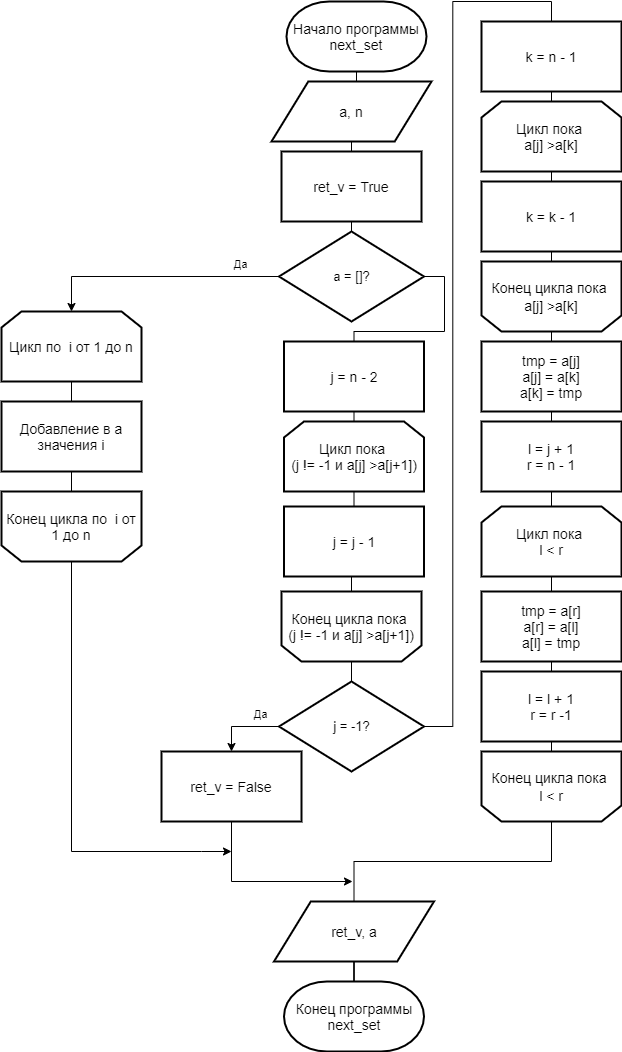
\includegraphics[scale=0.6]{inc/img/next_set.png}}
	
	\caption{Схема вспомогательной функции next\_set}
	
	\label{fig:next_set}
	
\end{figure}

\clearpage
На рисунке \ref{fig:count_len} приведена cхема вспомогательной функции count\_way\_len, которая с помощью матрицы смежности D вычисляет длину пути при проходе по городам visited\_cities.


\begin{figure}[h!]
	
	\centering{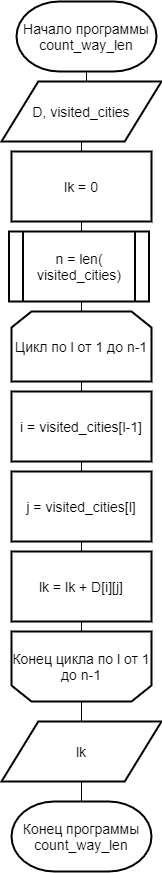
\includegraphics[scale=0.7]{inc/img/count_len.png}}
	
	\caption{Схема вспомогательной функции count\_way\_len}
	
	\label{fig:count_len}
	
\end{figure}

\clearpage
На рисунке \ref{fig:full_search} приведена cхема алгоритма полного перебора для решения задачи коммивояжера.

\clearpage
\begin{figure}[h!]
	
	\centering{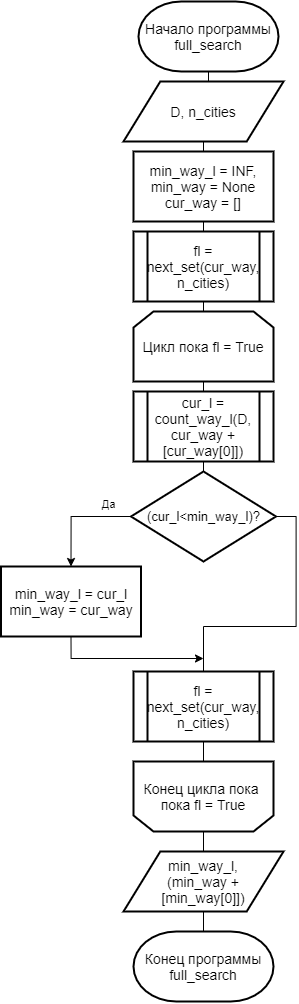
\includegraphics[scale=0.7]{inc/img/full_search.png}}
	
	\caption{Схема алгоритма полного перебора}
	
	\label{fig:full_search}
	
\end{figure}


\clearpage
\section{Схема муравьиного алгоритма}

На рисунке \ref{fig:ant_search} приведена схема муравьиного алгоритма для решения задачи коммивояжера.

\begin{figure}[h!]
	
	\centering{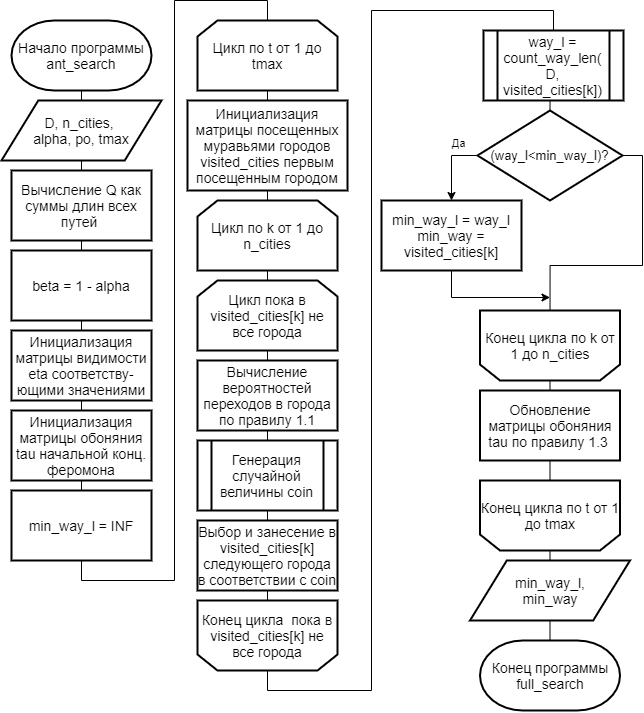
\includegraphics[scale=0.7]{inc/img/ant_search.png}}
	
	\caption{Схема муравьиного алгоритма}
	
	\label{fig:ant_search}
	
\end{figure}


\clearpage
\section{Вывод из конструкторской части}

Были приведены схемы разрабатываемых алгоритмов.


